\documentclass[a4paper, 10pt]{article}

\usepackage[english]{babel}
\usepackage[latin1]{inputenc}
\usepackage{empheq, amsmath, amssymb, amsthm, amssymb, indentfirst, setspace, hyperref, graphics, graphicx, verbatim, pgfplots, listings, xcolor, multicol}
\usepackage[super]{nth}
\usepackage[ruled, linesnumbered]{algorithm2e}
\usepackage{tikz}
\usetikzlibrary{arrows,calc}

\newtheorem{theorem}{Theorem }[section]
\newtheorem{definition}{Definition }[section]

\begin{document}

\begin{titlepage}
	\centering
	\begin{figure}[h!]
		\centering
		
\includegraphics[width=4cm]{Figures/cs}
	\end{figure}
	\vspace{4cm}
	{\scshape\Huge Applications of\\ quantum calculus\par}
	\vspace{1cm}
	{\Large Project Long \nth{2} year\par}
	\vspace{3cm}
	{\large Ahmed Ben Aissa\\
			Elie Mokbel\\
			Henrique Miyamoto\\
			Pierre Minssen\par}
	\vspace{2cm}
	{\large Prof. Beno�t Valiron \par}
	\vfill
	\large \today
\end{titlepage}

%\tableofcontents

%\title{Applications of quantum calculus}
%\author{Ahmed Ben Aissa, Elie Mokbel, Henrique Miyamoto, Pierre Minssen}
%\date{}
%\maketitle

\section{Basic concepts}

Classical computers operate on strings of bits (0 or 1) and produce other strings of bits. Classical data is supposed to be clonable, erasable, readable and not supposed to change when left untouched.

In quantum computation, on the other hand, the bits are replaced by \textit{quantum bits} or \textit{qubits}, which are unitary elements of the 2-dimensional complex Hilbert space $\mathbb{C}^2$. We choose the orthonormal basis called \textit{computational basis}
$$ |0\rangle = \begin{pmatrix} 1 \\0 \end{pmatrix} \text{ and } |1 \rangle = \begin{pmatrix} 0 \\1 \end{pmatrix}. $$

A general qubit can be seen a superposition of states $|0\rangle$ and $|1\rangle$
$$ |\psi\rangle = \alpha|0\rangle + \beta|1\rangle, $$
where $\alpha,\beta\in\mathbb{C}$.

The Hilbert space $\mathbb{C}^2$ is provided with an \textit{inner product} $\langle\varphi|\psi\rangle = {|\varphi\rangle}^{\dagger}|\psi\rangle = \sum_i\overline{\varphi}_i\psi_i$, which allows one to the define the \textit{norm} of a state $\||\psi\rangle\|=\sqrt{\langle\psi|\psi\rangle}$ and \textit{orthogonality} between two states when $\langle\varphi|\psi\rangle=0$.

\paragraph{Bloch spehre.} The Bloch sphere is a representation of quantum states on $S^2$. Let us consider the qubit in state $|\psi\rangle = \alpha|0\rangle + \beta|1\rangle$ and the polar representations $\alpha=|\alpha|e^{i\gamma}=\cos\frac{\theta}{2}e^{i\gamma}$ and $\beta=|\beta|e^{i(\gamma+\varphi)}=\sin\frac{\theta}{2}e^{i(\gamma+\varphi)}$. Then, we can write $|\psi\rangle=e^{i\gamma}\left(\cos\frac{\theta}{2}|0\rangle+e^{i\varphi}\sin\frac{\theta}{2}|1\rangle\right)$. Neglecting the global phase factor $e^{i\gamma}$\footnote{One reason for doing so is that this factor does not change the modulus squared of amplitudes $|\alpha|^2$ and $|\beta|^2$ \cite{portugal}.}, we have the mapping
$$ (\theta,\varphi) \mapsto \left(\cos\frac{\theta}{2},\ e^{i\varphi}\sin\frac{\theta}{2}\right), $$
with $\theta\in[0\,\pi]$ and $\varphi\in[0,2\pi[$.

\begin{figure}[h!]
	\centering
	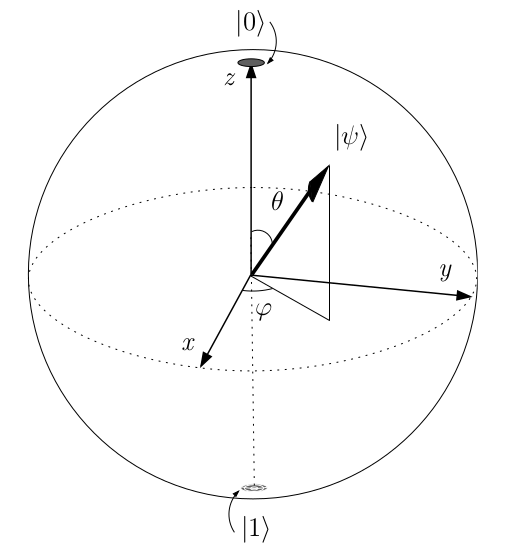
\includegraphics[width=5cm]{Figures/bloch}
	\caption{Bloch sphere \cite{portugal}.}
\end{figure}

\paragraph{Measurements.} It is a probabilistic operation that allows one to recover some classical information. The measurement of $|\psi\rangle = \alpha|0\rangle + \beta|1\rangle$ returns $|0\rangle$ with probability $|\alpha|^2$ and $|1\rangle$ with probability $|\beta|^2$. It also alters the state of a qubit and forces it to collapse to state $|0\rangle$ or $|1\rangle$, respectively. In this case, we say the measurement was done against the computational basis $\{|0\rangle,|1\rangle\}$.

\paragraph{Unitary operations.}  The temporal evolution of an isolated quantum system is described by linear transformations, represented by matrices. Transformations that map unitary vector onto unitary vectors are called \textit{unitary transformations} $U$ and can be defined by the following property:
$$ U^{\dagger}U = UU^{\dagger} = I, $$
where $U^{\dagger} = \left(\overline{U}\right)^T$ is the adjoint matrix and $I$ is the identity. These are reversible operations. 

Some usual gates are NOT, Hadamard, phase-shift and phase-flip:

\begin{itemize}
	\item NOT
	$$ N = \begin{pmatrix}
	0 & 1\\
	1 & 0
	\end{pmatrix} $$
	\item Hadamard
	$$ H = \frac{1}{\sqrt{2}}\begin{pmatrix}
	1 & 1\\
	1 & -1
	\end{pmatrix} $$
	\item Phase-shift
	$$ V_\theta = \begin{pmatrix}
	1 & 0\\
	0 & e^{i\theta}
	\end{pmatrix} $$
	\item Phase-flip\footnote{In fact, $Z$ is just $V_\pi$.}
	$$ Z = \begin{pmatrix}
	1 & 0\\
	0 & -1
	\end{pmatrix} $$
\end{itemize}

\paragraph{Tensor product.} The tensor product between two states
$$|\psi\rangle = \begin{pmatrix}
\psi_1\\
\vdots\\
\psi_m
\end{pmatrix}
\text{ and }
|\varphi\rangle = \begin{pmatrix}
\varphi_1\\
\vdots\\
\varphi_p
\end{pmatrix}$$
is computed as
$$
|\psi\rangle \otimes |\varphi\rangle = 
\begin{pmatrix}
\psi_1\varphi_1\\
\vdots\\
\psi_1\varphi_p\\
\psi_2\varphi_1\\
\vdots\\
\psi_2\varphi_p\\
\vdots\\
\psi_m\varphi_1\\
\vdots\\
\psi_m\varphi_p\\
\end{pmatrix}.
$$

In general, given two matrices $A\in\mathbb{C}^{m \times n}$ and $B\in\mathbb{C}^{p \times q}$, the tensor product is the matrix $A\otimes B\in\mathbb{C}^{mp \times nq}$ given by
$$ A\otimes B = \begin{pmatrix}
a_{11}B & a_{12}B & \cdots & a_{1n}B\\
a_{21}B & a_{22}B & \cdots & a_{2n}B\\
\vdots & \vdots & \ddots & \vdots\\
a_{m1}B & a_{m2}B & \cdots & a_{mn}B\\
\end{pmatrix} $$
where $a_{ij}$ is the $(i,j)$-element of $A$.

Given two linear transformations $A$ and $B$, we can define a new linear mapping by
$$ (A \otimes B)(|u\rangle \otimes |v\rangle) = A|u\rangle \otimes B|v\rangle. $$

Notation:
\begin{itemize}
	\item We can indistinguishably write $|\psi\rangle \otimes |\varphi\rangle = |\psi\rangle|\varphi\rangle = |\psi,\varphi\rangle = |\psi\varphi\rangle$.
	\item $|\psi\rangle^{\otimes n} = \underbrace{|\psi\rangle \otimes \cdots |\psi\rangle}_{n \text{ times}}$ and $A^{\otimes n} = \underbrace{A \otimes \cdots A}_{n \text{ times}}$.
\end{itemize}


\paragraph{Two or more qubits systems.} The state of a 2-qubit is an element of the tensor product space $\mathbb{C}^4 = \mathbb{C}^2 \otimes \mathbb{C}^2$, which is spanned by
$$|00\rangle = \begin{pmatrix}1\\0\\0\\0\end{pmatrix},\quad |10\rangle = \begin{pmatrix}0\\1\\0\\0\end{pmatrix},\quad |01\rangle = \begin{pmatrix}0\\0\\1\\0\end{pmatrix},\quad |11\rangle = \begin{pmatrix}0\\0\\0\\1\end{pmatrix}.$$

A generic state of 2 qubits it therefore of the form
$$ |\psi\rangle = \alpha|00\rangle + \beta|01\rangle + \gamma|10\rangle + \delta|11\rangle $$
with $|\alpha|^2+|\beta|^2+|\gamma|^2+|\delta|^2=1$.

In general, writing states as the decimal number correspoding to the binary representation (e.g. $|11\rangle \rightarrow |3\rangle$), a $n$-qubit state is described as
$$ |\psi\rangle = \sum_{i=0}^{2^n-1}\alpha_i|i\rangle, \text{ with } \sum_{i=0}^{2^n-1}|\alpha_i|^2=1. $$

As a generalisation of the 1-qubit case, the measurement of a $n$-qubit state changes it and forces it to collapse to one of the possible $|i\rangle$ states, each of which is measured with probability $|\alpha_i|^2$.

Among unitary operations available to 2-qubits states, we have the swap gate $X$ and the control-not gate $N_C$:
$$ X = \begin{pmatrix}
1 & 0 & 0 & 0\\
0 & 0 & 1 & 0\\
0 & 1 & 0 & 0\\
0 & 0 & 0 & 1\\
\end{pmatrix},\quad
N_C = \begin{pmatrix}
1 & 0 & 0 & 0\\
0 & 1 & 0 & 0\\
0 & 0 & 0 & 1\\
0 & 0 & 1 & 0\\
\end{pmatrix}. $$

The control-not gate changes the state of the second qubit only if the first qubit is in the state $|1\rangle$. It implements the mapping $|xy\rangle \mapsto |x\rangle \otimes |x\oplus y\rangle$.

The Toffoli gate acts on 3 qubits and is a ``control-control-not'': it implements the function $|xyz\rangle \mapsto |xy\rangle \otimes |z\oplus xy\rangle$, i.e., it changes the state of the last qubit if the two first qubits are in state $|11\rangle$.

\paragraph{Quantum entanglement.} Consider the states $|\psi\rangle = a|0\rangle + b|1\rangle$ and $|\varphi\rangle = c|0\rangle + d|1\rangle$. Their tensor product is $|\psi\varphi\rangle = ac|00\rangle + ad|01\rangle + bc|10\rangle + bd|11\rangle$. It turns out that a general state is not on this form, unless it has $\alpha\delta = \beta\gamma$.

We say a quantum state is \textit{entangled} when it cannot be written as a tensor product of two other states. For example, $\frac{1}{\sqrt{2}}(|00\rangle+|11\rangle)$ cannot have such a decomposition, and hence is an entangled state.

\paragraph{Quantum circuits} Quantum circuits are graphical representations of a procedure, i.e., a sequence of logical operations performed on a system. Unlike classical circuits, the wires must not be regarded as physical connections and their components are not available ``on the shelf''.

\begin{figure}[h!]
	\centering
	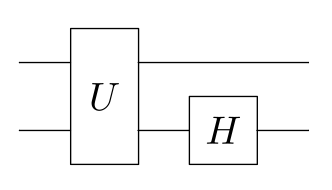
\includegraphics[width=4cm]{Figures/circuit}
	\caption{Example of quantum circuit representing $|\psi\rangle \mapsto (I\otimes H)(U|\psi\rangle)$ \cite{valiron}.}
\end{figure}

\section{Shor's algorithm}

The advantage of quantum algorithms over classical ones appears when using some quantum property such as entanglement or the interference, brought by complex coefficients.

In fact, quantum algorithms are based on a few ``real'' quantum constructions, such as quantum Fourier transform, quantum walk and amplitude amplification. The rest is composed of classical analysis and possibly an \textit{oracle}: a quantum circuit corresponding to a reversible operation.

Some interesting problems in algebra and number theory reduce to the problem of order finding. For example, the problem of factorising an integer number, which is addressed by Shor's algorithm.

\paragraph{Factorisation.} The objective of the \textit{factorisation problem} is to factorise a big number $N$ into prime numbers. Note that at least $n=\lceil\log_2N\rceil$ qubits are needed to store $N$ and that $n$ is the maximum number of prime factors. We will show how this problem reduces to the problem of finding the order of a randomly generated integer $x<N$ generated randomly.

If $N$ is even, 2 is trivially a factor. In addition, if $x$ and $N$ have common factors, then $\gcd(x,N)$ gives a factor of $N$; so we focus on investigating the case when $x$ and $N$ are coprimes.

\begin{definition}
	The order of $x$ modulo $N$ is the least positive integer $r$ such that
	$$ x^r \equiv 1 \mod N. $$
\end{definition}

\begin{theorem}[Euler's Theorem]
	If $x$ and $N$ are coprime positive integers, then
	$$ x^{\varphi(N)} \equiv 1 \mod N, $$
	where $\varphi(N)$ is the Euler's totient function, i.e., it indicates the number of coprimes to $N$ which are less or equal to it.
\end{theorem}

The \textit{order finding problem} is to find $r$, given $x$ and $N$ coprimes. The algorithm is built up on the following two theorems.

\begin{theorem}
	Let $N$ be a composite number stored with $n$ qubits and $x$ be non-trivial solution of the equation $x^2 \equiv 1 \mod N$ in the range $1 \le x \le N$, i.e., $x \not\equiv \pm 1 \mod N$. Then at least one of $\gcd(x+1,N)$ and $\gcd(x-1,N)$ is a non-trivial factor of $N$.
\end{theorem}

\begin{proof}
	Note that $x^2 \equiv 1 \mod N \Leftrightarrow x^2-1 \equiv 0 \mod N \Leftrightarrow (x+1)(x-1) \equiv 0 \mod N$, which means that $N$ is a divisor of $(x+1)(x-1)$. If $1<x<N-1$, then $0<x-1<x+1<N$ and $N$ cannot be a divisor of $(x+1)$ neither of $(x-1)$ separately. So both $(y+1)$ and $(y-1)$ must have factors of $N$. In this case, at least one of $\gcd(y+1,N)$ and $\gcd(y-1,N)$ produce a non-trivial factor of $N$\footnote{Such factor can be computed by using Euclid's algorithm.}.
\end{proof}

\begin{theorem}
	Suppose $N = p_{1}^{\alpha_1}...p_{m}^{\alpha_m}$ is the prime factorisation of and odd composite positive integer. Let $x$ be an integer chose uniformly at random such that $1 \le x\le N-1$ and $\gcd(x,N)=1$. Let $r$ be the order of $x$ modulo $N$. Then
	$$ \text{Pr}\{\text{$r$ is even and $x^{r/2}\not\equiv\pm1\mod N$}\} \ge 1-\frac{1}{2^m}. $$
\end{theorem}

\begin{proof}
	See \cite{ekert}, p. 751-752.
\end{proof}

The algorithm runs as follows.

\begin{algorithm}[h!]
	\caption{Shor's algorithm for factorising $N$.}
	If $N$ is even, return the factor 2.\\
	Randomly choose $x$ such that $1 \le x \le N-1$.\\
	If $\gcd(x,N)\neq1$, return the factor $\gcd(x,N)$.\\
	Find the order $r$ of $x$ modulo $N$.\\
	If $r$ is even and $x^{r/2}\not\equiv\pm 1\mod N$, then $\gcd(x^{r/2}+1)$ and $\gcd(x^{r/2}-1)$ are non-trivial factors.\\
	Else, restart the algorithm.
\end{algorithm}

Some remarks:

\begin{itemize}
	\item The method fails if $N$ is the power of a prime number. But in this case there exists a a classical algorithm to solve the problem \cite{portugal}. %Which one?
	\item The problem is finding the order of $x$ modulo $N$, for which there is no efficient classical procedure available. This problem is addressed in the next part.
\end{itemize}

\paragraph{Order finding.} The problem of order finding, i.e., given $x$ and $N$ coprimes, to find $r$ such that $x^r \equiv 1 \mod N$ is related to the matrix eigendecomposition. An unitary $U$, being a Hermitian matrix, can be decomposed as
$$ U=\sum_j \lambda_ju_ju_j^\dagger, $$
where $u_j$ are orthonormal eigenvectors and $\lambda_j$ are the associated eigenvalues.

Let us assume that $N=2^n$ and consider the operation $U_a$ on $n$ qubits that implements the mapping
$$U : \quad |j\rangle \mapsto |j\cdot x\mod N\rangle.$$
The operator is unitary because $x$ and $N$ are coprimes and the image of $\{0,...,N-1\}$ is the whole set. In particular, $U^k$ sends $|j\rangle \mapsto |j\cdot x^k \mod N\rangle$, so if $x^r \equiv 1 \mod N$, the map $U^r$ is the identity map.

The eigenstates of $U$ are of the form
$$ |u_s\rangle = \frac{1}{\sqrt{r}} \sum_{k=0}^{r-1}\exp{\left(-\frac{2\pi i sk}{r}\right)}|x^k \mod N \rangle $$
for $0 \le s \le r-1$. The eigenvalues are the $r$-th roots of the unity, having the form $e^{2\pi is/r}$, since
$$ U|u_s\rangle = \exp\left(\frac{2\pi is}{r}\right)|u_s\rangle. $$

An algorithm for finding such eigenvalues should be enough to find the order $r$ of $x$ modulo $N$\footnote{An alternative unitary could have been used: $V|j\rangle|k\rangle=|j\rangle|k+x^j\mod N\rangle$.}.

\paragraph{Quantum Fourier transform.} The quantum Fourier transform (QFT) is the operation
$$ |x\rangle \mapsto \frac{1}{\sqrt{2^n}}\sum_{y=0}^{2^n-1}e^{2\pi i\frac{x}{2^n}y}|y\rangle. $$
Its inverse is $\mathrm{QFT}^{-1}: \frac{1}{\sqrt{2^n}}\sum_{y=0}^{2^n-1}e^{2\pi i\frac{x}{2^n}y}|y\rangle \mapsto |x\rangle$ and will help solving the problem.

For the quantum phase estimation, we want to estimate $\omega$ in the state $|\phi\rangle = \frac{1}{\sqrt{2^n}}\sum_{y=0}^{2^n-1}e^{2\pi i\omega y}|y\rangle$. Without loss of generality, we will consider $\omega\in[0,1[$\footnote{We can do so because $e^{2\pi i}=1$.} and then decompose it as a floating number in binary notation: $\omega = \sum_{i=1}^{\infty}\frac{x_i}{2^i}$ or $\omega = 0.x_1x_2x_3...$ ($x_i\in\{0,1\}$).

\begin{itemize}
	\item If $\omega=0.x_1$ ($n=1$), we have $|\phi\rangle = \frac{1}{\sqrt{2}}\sum_{y=0}^{1}e^{\pi i (x_1y)}|y\rangle$ and we can retrieve $\omega$ by computing $H|\phi\rangle = |x_1\rangle$.
	\item If $\omega=0.x_1x_2$ ($n=2$), we can write $|\phi\rangle=\frac{1}{2}(|0\rangle+e^{2\pi i(0.x_2)}|1\rangle)\otimes(|0\rangle+e^{2\pi i(0.x_1x_2)}|1\rangle)$. To retrieve $\omega$, we consider $R_2 = \begin{pmatrix} 1 & 0\\ 0 & e^{2\pi i(0.01)} \end{pmatrix}$ and use the circuit
	\begin{figure}[h!]
		\centering
		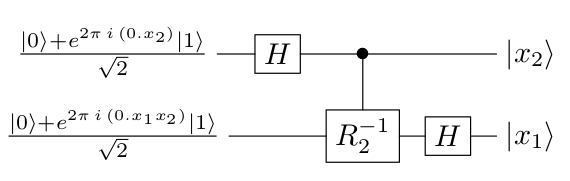
\includegraphics[width=6cm]{Figures/omega1}
	\end{figure}
	\item In general, it is possible to compute $|x_n...x_1\rangle$ from $|\phi\rangle$ by setting $R_n = \begin{pmatrix} 1 & 0\\ 0 & e^{2\pi i(0.0...01)} \end{pmatrix}$ and using the circuit
	\begin{figure}[h!]
		\centering
		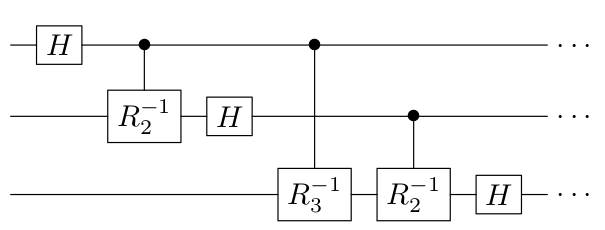
\includegraphics[width=6cm]{Figures/omega2}
	\end{figure}
\end{itemize}

\paragraph{Quantum phase estimation.} Suppose a unitary operator $U$ has an eigenvector $|u\rangle$ with eigenvalue $e^{2\pi i\varphi}$, where $\varphi$ is unknown. The objective of the \textit{phase estimation subroutine} is to estimate the value of $\varphi$. We assume we have oracles capable of preparing the state $|u\rangle$ and performing controlled-$U^{2^j}$ operations.

The procedure uses two registers: the first contains $t$ qubits initially in state $|0\rangle$. The number $t$ depends on the desired accuracy for $\varphi$ and on the probability we want the procedure to be successful. The second register begins with the state $|u\rangle$ and contains as many qubits as necessary to store it.

The first step is to apply the following circuit to the registers.

\begin{figure}[h!]
	\centering
	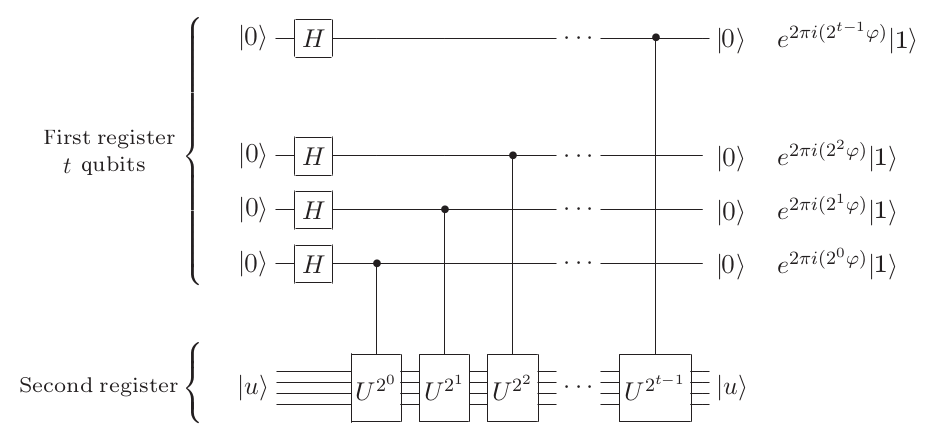
\includegraphics[width=10cm]{Figures/phase-estimation-1}
	\caption{Quantum circuit for first step of phase estimation (normalisation has been omitted on the right side) \cite{nielsen} .}
\end{figure}

The final state of the first register is
\begin{align*}
	&\frac{1}{2^{t/2}}\left(|0\rangle+e^{2\pi i2^{t-1}\varphi}|1\rangle\right)\left(|0\rangle+e^{2\pi i2^{t-2}\varphi}|1\rangle\right) \dots \left(|0\rangle+e^{2\pi i2^{0}\varphi}|1\rangle\right)\\
	=\ &\frac{1}{2^{t/2}}\sum_{k=0}^{2^t-1}e^{2\pi i\varphi k}|k\rangle.
\end{align*}

The second step is to apply the inverse Fourier transform on the first register and the third step is to measure it. Note that, if we write the previous expression using the binary fraction representation, we have
$$ \frac{1}{2^{t/2}}\left(|0\rangle+e^{2\pi i0.\varphi_t}|1\rangle\right)\left(|0\rangle+e^{2\pi i0.\varphi_{t-1}\varphi_{t}}|1\rangle\right) \dots \left(|0\rangle+e^{2\pi i0.\varphi_1...\varphi_t}|1\rangle\right). $$
Comparing it with the expression for the Fourier transform, one can see that the result of applying the inverse Fourier transform is the state $|\varphi_1\dots\varphi_r\rangle$ and a measurement in the computational basis gives exactly an estimation for $\varphi$!

\begin{figure}[h!]
	\centering
	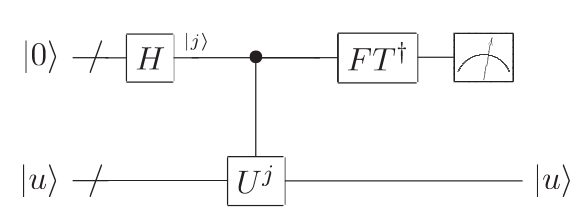
\includegraphics[width=6cm]{Figures/phase-estimation-2}
	\caption{Schematic of the overall phase estimation subroutine \cite{nielsen} .}
\end{figure}

Summarising, the phase estimation subroutine gives an estimation $\tilde{\varphi}$ to the phase of an eigenvalue of a unitary $U$, which is precisely what we wanted to implement the order finding algorithm. The inverse Fourier transform performs
$$ \frac{1}{2^{t/2}}\sum_{j=0}^{2^{t-1}}e^{2\pi i\varphi j}|j\rangle|u\rangle \mapsto |\tilde{\varphi}\rangle|u\rangle. $$

\begin{theorem}[Accuracy of $\varphi$ \cite{nielsen}]
	To successfully obtain $\varphi$ accurate to $n$ bits with probability of success at least $1-\epsilon$, we choose
	$$ t = n + \left\lceil \log\left(2+\frac{1}{2\epsilon}\right) \right\rceil. $$
\end{theorem}

TO DO:
\begin{itemize}
	\item Requirements for using phase estimation in order finding
	\item Continued fractions
\end{itemize}

\section{Implementation}

The implementations will be made using \textit{ProjectQ} \cite{projectq, steiger}.

TO DO: Adder \cite{draper}.

\begin{thebibliography}{10}

%\bibitem{mermin} Mermin, N. David. \textit{Quantum computer science: an introduction}. Cambridge: Cambridge University Press, 2007. 

\bibitem{valiron} Valiron, B. ``Quantum computation: a tutorial''. \textit{New Generation Computing}, vol. 30, issue 4, pp. 271-296, oct. 2012.

\bibitem{portugal} Portugal, R. et al. \textit{Uma introdu��o � computa��o qu�ntica}. S�o Carlos: SBMAC, 2004.

\bibitem{projectq} ProjectQ. Availabe in: \url{https://projectq.ch/}. Access on: 28 nov. 2018.

\bibitem{steiger} Steiger, Damian S.; H�ner, Thomas and Troyer, Matthias. ``ProjectQ: an open source software framework for quantum computing''. \textit{Quantum}, vol. 2, p. 49, jan. 2018.

\bibitem{nielsen} Nielsen, Michael A and Chuang, Isaac L. \textit{Quantum computation and quantum information}. 10th anniversary edition. Cambridge: Cambridge University Press, 2010.

\bibitem{ekert} Ekert, A. and Jozsa, R. ``Quantum computation and Shor's factoring algorithm''. \textit{Reviews of Modern Physics}, vol. 68, no. 3, pp. 733-753, 1996.

\bibitem{draper} Draper, Thomas G. \textit{Addition on a quantum computer}. Available in: \url{https://arxiv.org/abs/quant-ph/0008033}. Access on: 14 dec. 2018.

\end{thebibliography}

\end{document}